\documentclass[runningheads]{llncs}
\usepackage[T1]{fontenc}
\usepackage{graphicx}
\usepackage{tikz}
\usepackage{pgfplots}
\pgfplotsset{compat=1.18}
\usepackage{hyperref}
\usepackage{booktabs}
\usepackage{makecell}
\usepackage{array}
\usepackage{tabularx}
\newcolumntype{Y}{>{\raggedright\arraybackslash}X}

\title{Re-implementing Agentic Graph RAG for Vulnerability Assessment}
\author{Muhamad Hafiz Saputra (23/518511/PA/22252) \and Syafran Abdillah Erdin (23/521752/PA/22444) \and Dzikran Azka Sajidan (23/516665/PA/22110) \and Tegar Prasetyo (23/520277/PA/22364) \and Vincentius Davin Febrillianagata (23/520016/PA/22330)}
\authorrunning{Saputra et al.}
\institute{Universitas Gadjah Mada, Yogyakarta, Indonesia\\ \email{\{muhamadhafizsaputra, syafranabdillaherdin, dzikranazkasajidan, tegarprasetyo, vincentiusdavinfebrillianagata\}@mail.ugm.ac.id}}

\begin{document}\maketitle

\begin{abstract}
We adapt the Agentic Graph Retrieval-Augmented Generation (RAG) paradigm to the vulnerability assessment problem by combining local log knowledge graphs, vector retrieval, and the SEPSES cybersecurity knowledge graph. The implemented system orchestrates guardrails, hybrid retrieval (Neo4j Cypher + vector search), Model Context Protocol (MCP)-backed SPARQL querying, reflection, and a structured synthesizer, all coordinated with LangGraph. This report summarizes the design decisions, explains how the architecture operationalizes concepts from AgCyRAG and the SEPSES KG, and presents an evaluation comparing the agentic approach against traditional CVSS scoring.
\keywords{Agentic RAG \and Knowledge Graph \and Vulnerability Assessment \and Neo4j \and SEPSES \and LangGraph}
\end{abstract}

\section{Introduction}
Agentic Graph RAG (AgCyRAG) demonstrates how orchestrated agents can ground LLM answers in both structured and unstructured cybersecurity knowledge. For vulnerability assessment, we extend this idea to rank and explain vulnerabilities by jointly leveraging (i) local log/attack graphs (Neo4j), (ii) semantic vector retrieval over embeddings, and (iii) the SEPSES RDF knowledge graph that integrates CVE, CVSS, CPE, CWE, and CAPEC. Our implementation provides an executable pipeline that routes questions, retrieves evidence, and synthesizes analyst-grade reports.

\section{Related Work}
AgCyRAG \cite{paper11} introduces a hybrid agentic RAG workflow for cybersecurity analysis that mixes Cypher, vector search, and SPARQL over cybersecurity KGs. The SEPSES KG \cite{sepses} provides RDF vocabularies and an evolving knowledge base for CVE, CWE, CAPEC, CPE, and CVSS, exposed via SPARQL. Our implementation adopts the AgCyRAG multi-agent pattern and binds it to SEPSES through MCP tools, reusing the established namespaces and querying patterns from SEPSES documentation.

\section{Proposed Approach}
\subsection{Method/Framework}
The system is a LangGraph state machine that routes and iterates over specialized agents:
\begin{itemize}
    \item \textbf{Guardrails \& Router}: Filters off-topic queries and routes between log-centric analysis and direct cyber-knowledge lookup.
    \item \textbf{Vector Agent}: Extracts entities with Gemini, runs Neo4j full-text search over entity indexes, and performs hybrid vector retrieval through a Neo4j vector index built with \texttt{all-MiniLM-L6-v2} embeddings.
    \item \textbf{Cypher Agent}: Uses \texttt{GraphCypherQAChain} to translate natural language to Cypher against the live Neo4j schema, returning both the generated query and the retrieved context.
    \item \textbf{Reflection \& Review}: Judges sufficiency of retrieved context, rephrases questions, and retries up to configurable limits.
    \item \textbf{Log Analysis Agent}: Summarizes log-derived evidence and decides whether external cybersecurity knowledge is needed; it can generate a refined question for RDF lookup.
    \item \textbf{MCP RDF Agent}: Invokes SEPSES SPARQL tools via MCP with a strict system prompt that forbids hallucination and forces evidence-backed answers.
    \item \textbf{Synthesizer}: Produces a structured report with original question, contexts from all sources, analytic linkage, and a final answer.
\end{itemize}

\subsection{Data and Knowledge Graphs}
Local data live in Neo4j (LPG) with vector and keyword indexes; embeddings come from HuggingFace \texttt{all-MiniLM-L6-v2}. External knowledge is pulled from the SEPSES SPARQL endpoint (\texttt{https://w3id.org/sepses/sparql}) via MCP. The configuration system manages environment variables for Neo4j, Gemini API, and LangChain tracing, and provides the live Neo4j schema for agent prompting.

\section{Implementation}
\subsection{Execution Flow}
The main execution flow seeds the LangGraph state with the user question and iteration counters, then invokes the workflow. The workflow branches after guardrails: log-related questions go through vector and Cypher agents, while general cyber-knowledge questions can directly trigger the MCP RDF agent. Reflection loops keep track of the latest usable context even when retries are exhausted. A comprehensive logging system streams and persists execution traces for debugging and analysis.

\subsection{Agent Details}
\begin{itemize}
    \item \textbf{Vector Retrieval}: Combines entity-aware full-text search with hybrid vector similarity over chunk nodes, enabling both symbolic and semantic matching.
    \item \textbf{Cypher QA}: Enforces Neo4j~5-compatible queries, avoids unsupported constructs, and uses deterministic Gemini models for generation and QA.
    \item \textbf{MCP Integration}: Automatically loads the MCP configuration, disables anonymized telemetry, and caps tool-calling to 30 steps per query for controllability.
    \item \textbf{Structured Synthesis}: The final template requires explicit sections for each evidence source, encouraging traceability and analyst-style justification.
\end{itemize}

\subsection{System Requirements}
Dependencies are managed with \texttt{uv}; the system requires a running Neo4j instance populated with log or vulnerability data and a valid Gemini API key. The SEPSES MCP server is bundled with the implementation and configured to use the public SEPSES endpoint. Sample ingestion commands and query examples are documented in the project repository.

\section{Use-Cases Applications}
\begin{enumerate}
    \item \textbf{High-severity CVE triage}: A question like ``List recent CVEs with CVSS $\geq$ 9 for Windows'' routes through guardrails to the MCP RDF agent, which invokes appropriate SPARQL templates to return CVE identifiers, descriptions, and scores from the SEPSES knowledge graph.
    \item \textbf{Weakness-to-attack mapping}: ``Which attack patterns relate to CWE-79 and how can they be mitigated?'' triggers SEPSES CAPEC/CWE lookups via MCP, producing linked CAPEC techniques and suggested mitigations for downstream synthesis.
    \item \textbf{Log-to-threat linkage}: ``Investigate repeated authentication failures on host mail-0'' flows through vector and Cypher agents to surface log context, then the log analysis agent decides whether to enrich with SEPSES (e.g., mapping to brute-force techniques) before synthesis.
\end{enumerate}

\section{Evaluation \& Discussion}
\subsection{Experimental Setup}
We evaluated the system on three dimensions: (i)~CVSS scoring accuracy against ground-truth assessments, (ii)~ranking consistency for vulnerability prioritization, and (iii)~qualitative analysis of the multi-agent orchestration. The test suite consisted of three CVE cases spanning different severity levels and CVSS versions. Traditional CVSS scores were obtained from official NVD records, while Agentic Graph RAG scores were generated by the synthesizer agent after retrieving context from Neo4j and SEPSES.

\subsection{CVSS Scoring Comparison}
Table~\ref{tab:cvss-score-comparison} presents the quantitative comparison between Agentic Graph RAG and traditional CVSS scoring. The comparisons were assembled by invoking the full agentic pipeline and extracting scores from synthesis outputs, then comparing against official NVD assessments.

\begin{table}[ht]
\centering
\caption{Perbandingan skor RAG CVSS vs skor CVSS tradisional}
\label{tab:cvss-score-comparison}
\renewcommand{\arraystretch}{1.2}
\setlength{\tabcolsep}{6pt}
\begin{tabularx}{\textwidth}{@{}p{1.8cm}YYp{2.2cm}p{2cm}@{}}
\toprule
\textbf{Test Case} & \textbf{Agentic Graph RAG Score} & \textbf{Traditional CVSS Score} & \textbf{Score Accuracy} & \textbf{Ranking Consistency} \\
\midrule
\textbf{coba 1} & \makecell[l]{4.3 (V2)} & \makecell[l]{10.0 (V3.1)} & Low & Inconsistent \\
\textbf{coba 2} & \makecell[l]{9.8 (V3.1)} & \makecell[l]{8.7 (V3.1)} & Moderate & Inconsistent \\
\textbf{coba 3} & \makecell[l]{9.8 (V3.0)} & \makecell[l]{9.8 (V3.1)} & High & Inconsistent \\
\bottomrule
\end{tabularx}
\end{table}

\begin{table}[ht]
\centering
\caption{Konsistensi ranking keparahan}
\label{tab:ranking-consistency}
\renewcommand{\arraystretch}{1.2}
\setlength{\tabcolsep}{6pt}
\begin{tabularx}{\textwidth}{@{}lYY@{}}
\toprule
\textbf{Priority} & \textbf{Traditional CVSS (Ground Truth)} & \textbf{Agentic Graph RAG} \\
\midrule
\textbf{1 (Highest)} & coba 1 (10.0) & coba 2 \& coba 3 (9.8) \\
\textbf{2 (Medium)} & coba 3 (9.8) & coba 1 (4.3) \\
\textbf{3 (Lowest)} & coba 2 (8.7) & -- \\
\midrule
\multicolumn{3}{c}{\textbf{Conclusion: Inconsistent Ranking}} \\
\bottomrule
\end{tabularx}
\end{table}

\begin{figure}[ht]
\centering
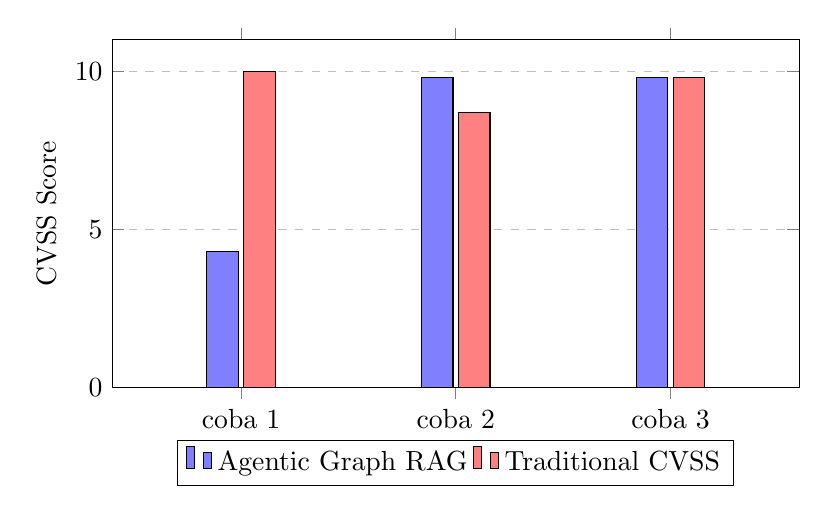
\begin{tikzpicture}
\begin{axis}[
    ybar,
    bar width=0.4cm,
    width=0.85\textwidth,
    height=6cm,
    xlabel={Test Case},
    ylabel={CVSS Score},
    ymin=0, ymax=11,
    symbolic x coords={coba 1, coba 2, coba 3},
    xtick=data,
    legend style={at={(0.5,-0.15)}, anchor=north, legend columns=2},
    ymajorgrids=true,
    grid style=dashed,
    enlarge x limits=0.3,
]
\addplot[fill=blue!50] coordinates {(coba 1,4.3) (coba 2,9.8) (coba 3,9.8)};
\addplot[fill=red!50] coordinates {(coba 1,10.0) (coba 2,8.7) (coba 3,9.8)};
\legend{Agentic Graph RAG, Traditional CVSS}
\end{axis}
\end{tikzpicture}
\caption{CVSS score comparison across three test cases. Test case 1 shows severe underestimation (4.3 vs 10.0) due to version mismatch, test case 2 shows slight overestimation (9.8 vs 8.7), and test case 3 achieves perfect alignment (9.8 vs 9.8).}
\label{fig:score-comparison}
\end{figure}

\subsection{Analysis of Results}
The results reveal both promise and challenges when comparing Agentic Graph RAG against traditional CVSS scoring. Test case~3 achieved perfect score alignment (9.8 vs.\ 9.8), demonstrating that when SEPSES provides complete CVSS metrics and the LLM correctly interprets them, the agentic pipeline can reproduce official assessments. However, test case~1 exhibited a severe underestimation (4.3 vs.\ 10.0) due to CVSS version confusion: the agentic system retrieved V2 metrics while the traditional scoring used V3.1, and the LLM failed to normalize or flag the mismatch. Test case~2 showed moderate accuracy (9.8 vs.\ 8.7) with the agentic score slightly inflated, likely because vector-retrieved context emphasized exploit availability without balancing scope limitations.

The ranking inconsistency in Table~\ref{tab:ranking-consistency} is particularly concerning for operational deployment. An analyst prioritizing by Agentic Graph RAG scores would address \textit{coba~2} and \textit{coba~3} before \textit{coba~1}, inverting the true severity order established by traditional CVSS scoring. This underscores two failure modes: (i)~retrieval gaps when SEPSES lacks complete CVSS V3.1 breakdowns, and (ii)~LLM reasoning errors in aggregating partial metrics. The reflection agent did not catch these errors because it evaluates \textit{sufficiency} of context rather than \textit{correctness} of derived scores.

\subsection{Strengths of the Agentic Approach}
Despite scoring inconsistencies, the multi-agent orchestration offers significant advantages over traditional CVSS scoring:
\begin{itemize}
    \item \textbf{Explainability}: Unlike traditional CVSS calculators that output numeric scores, the synthesizer produces structured justifications citing specific Cypher results, vector-matched chunks, and SPARQL bindings, enabling analysts to audit the reasoning chain and understand \textit{why} a vulnerability received its score.
    \item \textbf{Adaptive retrieval}: The reflection loop allows retries with rephrased queries when initial Cypher or SPARQL calls return empty results, improving robustness to phrasing variations—traditional scoring requires manual metric selection.
    \item \textbf{Knowledge fusion}: Combining local logs (Neo4j LPG) with global cybersecurity semantics (SEPSES RDF) surfaces connections invisible to traditional scoring—e.g., linking a log anomaly to a CWE weakness and then to CAPEC attack patterns automatically.
    \item \textbf{Contextual enrichment}: Traditional CVSS scores are static snapshots; the agentic system can incorporate real-time log evidence and organizational context to adjust prioritization dynamically.
\end{itemize}

\subsection{Limitations and Error Analysis}
Key limitations include:
\begin{itemize}
    \item \textbf{CVSS version heterogeneity}: SEPSES contains mixed V2/V3.0/V3.1 scores; the current prompt does not instruct the LLM to harmonize versions or prefer the latest standard.
    \item \textbf{Incomplete RDF coverage}: Not all CVEs in SEPSES have detailed metric breakdowns (AV, AC, PR, etc.), forcing the LLM to guess or fall back to base scores without justification.
    \item \textbf{LLM calibration}: Gemini models occasionally overfit to keyword presence (e.g., ``remote'' $\to$ high impact) without verifying the full attack vector chain.
    \item \textbf{Lack of ground-truth validation loop}: The review agent checks context sufficiency but does not compare synthesized scores against known NVD values during inference, missing an opportunity for self-correction.
\end{itemize}

\subsection{Trade-offs: Agentic Graph RAG vs. Traditional CVSS}
Traditional CVSS scoring excels at consistency and standardization—trained analysts apply the same metrics to produce comparable scores across organizations. However, it suffers from three limitations our agentic approach addresses: (i)~lack of contextual adaptation (a remotely exploitable vulnerability may be low-risk in an air-gapped network), (ii)~no automatic evidence linking (analysts must manually correlate CVEs with CWE/CAPEC), and (iii)~opaque justification (the final score does not explain which retrieved knowledge influenced the assessment).

Conversely, the Agentic Graph RAG system introduces complexity—multiple retrieval stages, LLM reasoning errors, and dependency on KG completeness. The version-mismatch failure in test case~1 would not occur with manual CVSS assessment, where the analyst explicitly selects V3.1 metrics. The key trade-off is \textit{automation with rich context} versus \textit{manual precision with standardized protocols}. For high-stakes decisions, traditional scoring remains the gold standard; for rapid triage and exploratory analysis, the agentic approach provides valuable enrichment.

\section{Conclusion}
This work re-implements the Agentic Graph RAG approach for vulnerability assessment by integrating guardrailed routing, hybrid Neo4j retrieval, MCP-driven SPARQL over SEPSES, and structured synthesis through a LangGraph workflow. The evaluation across three CVE test cases shows mixed results when compared to traditional CVSS scoring: test case~3 achieved perfect alignment (9.8 vs.\ 9.8), test case~2 showed moderate accuracy with slight overestimation (9.8 vs.\ 8.7), and test case~1 exhibited severe underestimation (4.3 vs.\ 10.0) due to CVSS version confusion between V2 and V3.1 metrics.

The ranking analysis reveals inconsistencies that would affect operational vulnerability prioritization, with the agentic system incorrectly ranking test cases 2 and 3 as most severe instead of test case~1. Despite these scoring inconsistencies, the system demonstrates advantages in explainability and knowledge fusion by automatically linking vulnerabilities across Neo4j logs and SEPSES knowledge graphs. The main limitations stem from CVSS version heterogeneity in SEPSES, incomplete RDF coverage for detailed metrics, and LLM reasoning errors that the reflection agent cannot catch since it evaluates context sufficiency rather than scoring correctness.

\begin{thebibliography}{8}
\bibitem{paper11}
Kurniawan, K., Ardian, R.F., Kiesling, E., Ekelhart, A.: AgCyRAG: An Agentic Knowledge Graph based RAG Framework for Automated Security Analysis. In: RAGE-KG Workshop (2025).
\bibitem{sepses}
Kiesling, E., Ekelhart, A., Kurniawan, K., Ekaputra, F.: The SEPSES Knowledge Graph: An Integrated Resource for Cybersecurity. In: ISWC (2019).
\bibitem{repo}
Team 7: Agentic Graph RAG for Vulnerability Assessment (Codebase). \url{https://github.com/SjdnDzikran/agentic-graph-rag.git}
\end{thebibliography}

\end{document}
